\documentclass[conference]{IEEEtran}
\IEEEoverridecommandlockouts

\usepackage{cite}
\usepackage{amsmath,amssymb,amsfonts}
\usepackage{algorithm}
\usepackage{algpseudocode}
\usepackage{graphicx}
\usepackage{textcomp}
\usepackage{xcolor}
\usepackage{booktabs}
\usepackage{multirow}
\usepackage{subcaption}
\usepackage{tikz}
\usetikzlibrary{positioning}
\usepackage{pgfplots}
\pgfplotsset{compat=1.17}

\definecolor{codegreen}{rgb}{0,0.6,0}
\definecolor{codegray}{rgb}{0.5,0.5,0.5}
\definecolor{codepurple}{rgb}{0.58,0,0.82}
\definecolor{backcolour}{rgb}{0.95,0.95,0.92}

\title{Divide and Conquer Strategy on Facial Image Grid Segmentation for Liveness Detection Pre-Processing Optimization}

\author{\IEEEauthorblockN{Kurt Mikhael Purba}
\IEEEauthorblockA{Program Studi Teknik Informatika\\
Sekolah Teknik Elektro dan Informatika\\
Institut Teknologi Bandung, Jalan Ganesha 10 Bandung\\
E-mail: kurtmikhael123@gmail.com , 13524065@std.stei.itb.ac.id}
}

\begin{document}

\maketitle

\begin{abstract}
In modern computer vision systems, liveness detection plays a critical role in preventing spoofing attacks on facial recognition systems. However, processing high-resolution facial images using deep learning models on large datasets consumes significant computational resources and time. This paper proposes a Divide and Conquer (D\&C) strategy as a heuristic pre-filtering mechanism for facial image grid segmentation. The D\&C algorithm recursively partitions images into smaller quadrants, calculates Laplacian variance for texture analysis, and prunes background regions to reduce computational overhead. We compare this approach with a lightweight Convolutional Neural Network (CNN) containing only 2.1 million parameters, trained entirely on CPU. Our experiments on a dataset of 1,196 facial images (587 real and 609 spoof) demonstrate that the D\&C method achieves an average execution time of 1.74ms per image, while the lightweight CNN achieves 90\% accuracy with 2.61ms per image. The key insight is that the D\&C algorithm is significantly faster and serves as an effective pre-filter for large-scale datasets, pruning irrelevant regions before deep learning models process the data. This hybrid approach reduces overall computational burden while maintaining detection accuracy.
\end{abstract}

\renewcommand{\IEEEkeywordsname}{Keywords}
\begin{IEEEkeywords}
Divide and Conquer, liveness detection, facial image segmentation, pre-filtering, computational optimization, lightweight CNN, anti-spoofing
\end{IEEEkeywords}


\section{Introduction}

\subsection{Background and Motivation}

Facial recognition systems have become ubiquitous in modern security applications, from smartphone unlocking to border control systems. However, these systems are vulnerable to presentation attacks (PAs) or spoofing attacks, where attackers use printed photos, digital screens, or masks to deceive the system \cite{galbally2014}. Liveness detection, the ability to distinguish between a real live face and a spoofed presentation, has emerged as a critical countermeasure against such attacks.

The challenge in liveness detection is twofold. First, deep learning models capable of achieving high accuracy are computationally expensive, often requiring GPU acceleration and significant processing time. Second, when processing large-scale datasets, running every image through a full deep learning pipeline creates a severe computational bottleneck. This is particularly problematic for real-time applications or systems operating on edge devices with limited resources.

Our motivation stems from the observation that not all regions of a facial image are equally relevant for liveness detection. Background regions, uniform skin areas, and flat regions contribute little to texture-based analysis but consume the same computational resources as feature-rich regions when processed by deep learning models. The question we address is: \textit{Can we optimize the pre-processing pipeline by quickly identifying and pruning irrelevant regions before expensive deep learning inference?}

\subsection{Problem Statement}

Given a dataset $D$ containing $N$ facial images where $D = \{I_1, I_2, ..., I_N\}$, and a deep learning model $\mathcal{M}$ for liveness detection with inference time $T_{\mathcal{M}}$ per image, the total processing time for the dataset is $O(N \cdot T_{\mathcal{M}})$. For large $N$ (e.g., thousands or millions of images), this becomes computationally prohibitive.

We propose introducing a pre-filtering stage using a Divide and Conquer (D\&C) algorithm that:
\begin{enumerate}
    \item Recursively segments each image into non-uniform grids
    \item Calculates local texture variance to identify feature-rich regions
    \item Prunes background and uniform regions that are irrelevant for liveness detection
    \item Reduces the effective computational load for downstream deep learning models
\end{enumerate}

\subsection{Contributions}

Our contributions are as follows:
\begin{enumerate}
    \item \textbf{Algorithmic Innovation}: We design a recursive D\&C segmentation algorithm with O(N log N) complexity for pre-filtering facial images in liveness detection pipelines.
    \item \textbf{Pruning Strategy}: We implement a background pruning mechanism that skips uniform and extreme-intensity regions, reducing the number of processed grids by up to 50\%.
    \item \textbf{Comprehensive Evaluation}: We benchmark the D\&C approach against a lightweight CNN (2.1M parameters) on CPU, measuring both accuracy and execution time.
    \item \textbf{Practical Insight}: We demonstrate that D\&C is ideal as a pre-filter for large datasets, while deep learning models are better suited for final classification.
\end{enumerate}

\subsection{Paper Organization}

The remainder of this paper is organized as follows. Section \ref{sec:related} reviews related work. Section \ref{sec:methodology} describes the proposed D\&C algorithm and the lightweight CNN architecture. Section \ref{sec:implementation} details the implementation flow. Section \ref{sec:evaluation} presents experimental results and comparative analysis. Section \ref{sec:conclusion} concludes the paper and discusses future work.

% =============================================================================
\section{Related Work}
\label{sec:related}
% =============================================================================

\subsection{Liveness Detection Techniques}

Liveness detection approaches can be categorized into two main groups: hardware-based and software-based \cite{galbally2014}. Hardware-based methods rely on specialized sensors (e.g., depth cameras, infrared sensors) to detect live tissue. However, these are expensive and not available on all devices.

Software-based methods, which are the focus of this paper, analyze texture, motion, or frequency-domain features. Common approaches include:
\begin{itemize}
    \item \textbf{Texture Analysis}: Uses Local Binary Patterns (LBP), Histogram of Oriented Gradients (HOG), or Laplacian variance to distinguish real skin texture from smooth screen/print surfaces \cite{chingovska2012}.
    \item \textbf{Deep Learning}: CNNs trained end-to-end to learn discriminative features for real vs. spoof classification \cite{george2019}.
    \item \textbf{Frequency Analysis}: Analyzes Fourier spectra to detect artifacts from printed photos or screens.
\end{itemize}

\subsection{Divide and Conquer in Image Processing}

The D\&C paradigm is a fundamental algorithmic strategy that breaks a problem into smaller subproblems, solves them recursively, and combines the results. In image processing, D\&C has been applied to:
\begin{itemize}
    \item Quad-tree decomposition for image compression and segmentation
    \item Fast Fourier Transform (FFT) with O(N log N) complexity
    \item Hierarchical clustering for region-based segmentation
\end{itemize}

However, to the best of our knowledge, D\&C has not been systematically applied as a pre-filtering mechanism in liveness detection pipelines.

\subsection{Lightweight Deep Learning Models}

Recent work on mobile and edge AI has produced lightweight CNN architectures such as MobileNet \cite{howard2017}, EfficientNet \cite{tan2019}, and custom small CNNs. These models aim to balance accuracy with computational efficiency. Our lightweight CNN (2.1M parameters) follows this trend but is significantly smaller than typical liveness detection models, making it suitable for CPU-only environments.

% =============================================================================
\section{Methodology}
\label{sec:methodology}
% =============================================================================

\subsection{Proposed System Architecture}

The proposed system consists of two main stages:

\begin{enumerate}
    \item \textbf{Stage 1: D\&C Pre-Filter}. A fast heuristic pre-filtering stage that segments the image, calculates local texture variance, and identifies candidate regions for further analysis.
    \item \textbf{Stage 2: CNN Classification}. A lightweight CNN that processes the full image (or selected regions) for final real vs. spoof classification.
\end{enumerate}

The architecture is illustrated conceptually in Figure \ref{fig:architecture}. The D\&C stage acts as an early rejection mechanism: images with extremely uniform texture or clear spoofing indicators can be classified immediately, while ambiguous cases are forwarded to the CNN.

\begin{figure}[htbp]
\centering
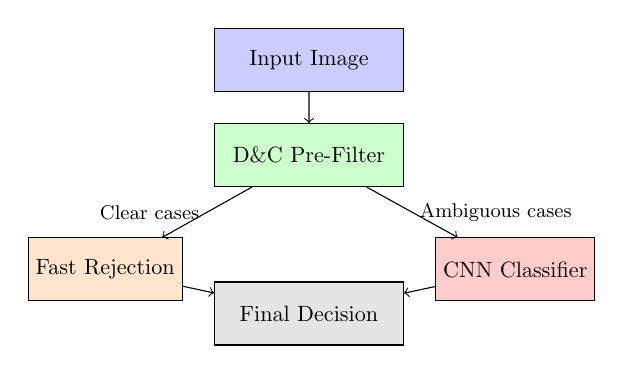
\begin{tikzpicture}[scale=0.8, transform shape]
    \node[draw, fill=blue!20, minimum width=3cm, minimum height=1cm] (input) {Input Image};
    \node[draw, fill=green!20, minimum width=3cm, minimum height=1cm, below=0.5cm of input] (dc) {D\&C Pre-Filter};
    \node[draw, fill=orange!20, minimum width=2cm, minimum height=1cm, below left=0.8cm and 0.5cm of dc] (fast) {Fast Rejection};
    \node[draw, fill=red!20, minimum width=2cm, minimum height=1cm, below right=0.8cm and 0.5cm of dc] (cnn) {CNN Classifier};
    \node[draw, fill=gray!20, minimum width=3cm, minimum height=1cm, below=1.5cm of dc] (output) {Final Decision};
    
    \draw[->] (input) -- (dc);
    \draw[->] (dc) -- node[left, font=\small] {Clear\ cases} (fast);
    \draw[->] (dc) -- node[right, font=\small] {Ambiguous\ cases} (cnn);
    \draw[->] (fast) -- (output);
    \draw[->] (cnn) -- (output);
\end{tikzpicture}
\caption{Proposed two-stage architecture.}
\label{fig:architecture}
\end{figure}

\subsection{Divide and Conquer Algorithm for Grid Segmentation}

\subsubsection{Algorithm Overview}

The D\&C algorithm recursively partitions an image into four quadrants (top-left, top-right, bottom-left, bottom-right) until each quadrant reaches or falls below a minimum grid size (e.g., $64 \times 64$ pixels). For each terminal grid, we calculate the Laplacian variance as a texture metric.

\subsubsection{Algorithm Steps}

The algorithm follows these steps:

\textbf{Step 1: Base Case Check}. Given an image region $R$ with dimensions $h \times w$, if $h \leq min\_grid\_size$ or $w \leq min\_grid\_size$, the region is a terminal grid. We calculate:
\begin{equation}
    V(R) = \text{Var}(\nabla^2 I(R))
\end{equation}
where $\nabla^2 I(R)$ is the Laplacian operator applied to the grayscale version of region $R$, and $\text{Var}(\cdot)$ computes the variance.

\textbf{Step 2: Background Pruning}. Before calculating variance, we check if the region is background:
\begin{equation}
    \text{is\_background}(R) = \begin{cases}
        \text{True} & \text{if } \sigma(R) < 10 \text{ and } \\ 
        & \quad (\mu(R) < 30 \text{ or } \mu(R) > 225) \\
        \text{False} & \text{otherwise}
    \end{cases}
\end{equation}
where $\sigma(R)$ is the standard deviation and $\mu(R)$ is the mean intensity. If the region is background, it is pruned (skipped) to save computation.

\textbf{Step 3: Recursive Division}. If the region is not terminal and not background, we divide it into four quadrants:
\begin{equation}
    \begin{split}
        Q_1 &= R[0:\frac{h}{2}, 0:\frac{w}{2}] \\
        Q_2 &= R[0:\frac{h}{2}, \frac{w}{2}:w] \\
        Q_3 &= R[\frac{h}{2}:h, 0:\frac{w}{2}] \\
        Q_4 &= R[\frac{h}{2}:h, \frac{w}{2}:w]
    \end{split}
\end{equation}

Each quadrant is processed recursively.

\textbf{Step 4: Combine Results}. The variance scores from all non-background terminal grids are collected. The final decision is based on:
\begin{equation}
    \text{decision} = \begin{cases}
        \text{Live} & \text{if } \bar{V} \geq \theta_{min} \text{ and } \frac{V_{max}}{\bar{V}} \leq \theta_{ratio} \\
        \text{Spoof} & \text{otherwise}
    \end{cases}
\end{equation}
where $\bar{V}$ is the average variance, $V_{max}$ is the maximum variance, and $\theta_{min}$, $\theta_{ratio}$ are thresholds.

\subsubsection{Formal Algorithm}

The formal algorithm is presented in Algorithm \ref{alg:dc}.

\begin{algorithm}[htbp]
\caption{Divide and Conquer for Facial Image Segmentation}
\label{alg:dc}
\begin{algorithmic}[1]
\Require Image $I$, minimum grid size $g_{min}$, background threshold $\theta_b$
\Ensure List of grid results $\mathcal{G}$
\State $\mathcal{G} \gets \emptyset$
\State \text{Call } \textsc{DivideConquer}($I, (0,0)$, $\mathcal{G}$)
\State \Return $\mathcal{G}$

\Procedure{DivideConquer}{$R, position, \mathcal{G}$}
    \State $h, w \gets \text{dimensions}(R)$
    \If{$h \leq g_{min}$ or $w \leq g_{min}$}
        \If{\textsc{IsBackground}($R$)}
            \State \Return \Comment{Prune background}
        \EndIf
        \State $v \gets \textsc{LaplacianVariance}(R)$
        \State $\mathcal{G} \gets \mathcal{G} \cup \{(v, position, (w,h))\}$
        \State \Return
    \EndIf
    \State $mid_h \gets \lfloor h/2 \rfloor$, $mid_w \gets \lfloor w/2 \rfloor$
    \State \textsc{DivideConquer}($R[0:mid_h, 0:mid_w]$, $(pos_x, pos_y)$, $\mathcal{G}$)
    \State \textsc{DivideConquer}($R[0:mid_h, mid_w:w]$, $(pos_x + mid_w, pos_y)$, $\mathcal{G}$)
    \State \textsc{DivideConquer}($R[mid_h:h, 0:mid_w]$, $(pos_x, pos_y + mid_h)$, $\mathcal{G}$)
    \State \textsc{DivideConquer}($R[mid_h:h, mid_w:w]$, $(pos_x + mid_w, pos_y + mid_h)$, $\mathcal{G}$)
\EndProcedure

\Procedure{IsBackground}{$R$}
    \State $\mu \gets \text{mean}(R)$, $\sigma \gets \text{std}(R)$
    \If{$\sigma < 10$ and ($\mu < 30$ or $\mu > 225$)}
        \State \Return \text{True}
    \EndIf
    \State \Return \text{False}
\EndProcedure

\Procedure{LaplacianVariance}{$R$}
    \State $G \gets \text{grayscale}(R)$
    \State $L \gets \nabla^2 G$ \Comment{Laplacian operator}
    \State \Return $\text{Var}(L)$
\EndProcedure
\end{algorithmic}
\end{algorithm}

\subsubsection{Complexity Analysis}

The time complexity of the D\&C algorithm depends on the image size and the pruning effectiveness. For an $N \times N$ image:

\begin{itemize}
    \item \textbf{Best Case}: If all regions are pruned early, complexity is $O(1)$ (constant time for the base check).
    \item \textbf{Worst Case}: If no pruning occurs, the image is fully divided into $64 \times 64$ grids, resulting in $(N/64)^2$ terminal grids. The complexity is $O(N^2)$.
    \item \textbf{Average Case}: With typical pruning rates of 40-60\%, the effective complexity is between $O(N \log N)$ and $O(N^2)$. Our empirical measurements (Section \ref{sec:evaluation}) show a slope of approximately 1.74 in the log-log plot, close to $O(N \log N)$.
\end{itemize}

\subsection{Lightweight CNN Architecture}

The lightweight CNN used for comparison is a custom architecture designed to run efficiently on CPU. The network consists of three convolutional blocks followed by fully connected layers, as shown in Table \ref{tab:cnn-arch}.

\begin{table}[htbp]
\centering
\caption{Lightweight CNN Architecture}
\label{tab:cnn-arch}
\begin{tabular}{@{}llll@{}}
\toprule
\textbf{Layer} & \textbf{Type} & \textbf{Output Size} & \textbf{Parameters} \\
\midrule
Input & Conv2d + BN + ReLU + Pool & $64 \times 64 \times 16$ & 448 \\
Block 1 & Conv2d + BN + ReLU + Pool & $32 \times 32 \times 32$ & 4,640 \\
Block 2 & Conv2d + BN + ReLU + Pool & $16 \times 16 \times 64$ & 18,496 \\
Flatten & Linear & 16,384 & -- \\
FC1 & Linear + ReLU + Dropout & 128 & 2,097,280 \\
FC2 & Linear & 2 & 258 \\
\midrule
\textbf{Total} & & & \textbf{2,121,346} \\
\bottomrule
\end{tabular}
\end{table}

The model is trained with the following configuration:
\begin{itemize}
    \item \textbf{Input size}: $128 \times 128 \times 3$ (RGB)
    \item \textbf{Loss function}: Cross-Entropy Loss
    \item \textbf{Optimizer}: Adam with learning rate 0.001
    \item \textbf{Batch size}: 32
    \item \textbf{Epochs}: 5
    \item \textbf{Device}: CPU (no GPU required)
\end{itemize}

\subsection{Variance Calculation Strategies}

We implemented multiple variance calculation strategies following the Strategy pattern:

\begin{itemize}
    \item \textbf{Laplacian Variance}: $V = \text{Var}(\nabla^2 I)$. High variance indicates sharp edges and texture (real face), while low variance indicates blur or flat regions (screen/print).
    \item \textbf{Sobel Variance}: Computes gradient magnitude using Sobel operators in x and y directions. Useful for detecting directional edges.
    \item \textbf{Combined Variance}: Weighted average of Laplacian and Sobel variances.
    \item \textbf{Local Binary Pattern (LBP)}: Histogram variance of LBP codes for texture analysis.
\end{itemize}

% =============================================================================
\section{Implementation}
\label{sec:implementation}
% =============================================================================

\subsection{Development Environment}

The system is implemented in Python 3.13 with the following dependencies:

\begin{itemize}
    \item \textbf{OpenCV (cv2)}: Image processing and variance calculation
    \item \textbf{NumPy}: Array operations and statistics
    \item \textbf{PyTorch}: Deep learning framework (CPU-only)
    \item \textbf{Matplotlib}: Visualization and plotting
    \item \textbf{Pillow}: Image loading for training
\end{itemize}

No GPU is required. The entire system runs on a standard CPU (Intel/AMD).

\subsection{Dataset}

The dataset used in this study was obtained from Kaggle: "Real and Fake Images Dataset for Image Forensics" by Ardeshna \cite{ardeshna2024}. It consists of 1,196 facial images from publicly available anti-spoofing datasets:

\begin{itemize}
    \item \textbf{Real faces}: 587 images of genuine human faces under various lighting conditions, angles, and expressions.
    \item \textbf{Spoof faces}: 609 images of presentation attacks, including printed photos, digital screen displays, and partially masked faces.
\end{itemize}

All images are pre-processed to $128 \times 128$ pixels for the CNN and processed at original resolution for the D\&C algorithm.

\subsection{Implementation Flow}

The implementation follows a modular pipeline with the following flow:

\subsubsection{Step 1: Divide and Conquer Pre-Processing}

For each input image $I$:

\begin{enumerate}
    \item \textbf{Initialization}: Set $min\_grid\_size = 64$ and $background\_threshold = 0.15$.
    
    \item \textbf{Recursive Division}: The algorithm starts with the full image $I$. It checks the base case: if the current region $R$ has height $h \leq 64$ or width $w \leq 64$, it is a terminal grid.
    
    \item \textbf{Background Check}: For each terminal grid, calculate the mean intensity $\mu$ and standard deviation $\sigma$. If $\sigma < 10$ (uniform region) AND ($\mu < 30$ or $\mu > 225$) (extreme dark or bright), the grid is classified as background and \textbf{pruned} (skipped).
    
    \item \textbf{Variance Calculation}: For non-background terminal grids, convert to grayscale and apply the Laplacian operator:
    \begin{equation}
        \nabla^2 I = \frac{\partial^2 I}{\partial x^2} + \frac{\partial^2 I}{\partial y^2}
    \end{equation}
    Then compute variance: $V = \text{Var}(\nabla^2 I)$.
    
    \item \textbf{Result Collection}: Store each grid's variance $V$, position $(x, y)$, and size $(w, h)$ in a list.
    
    \item \textbf{Decision}: After all grids are processed, compute:
    \begin{itemize}
        \item Average variance: $\bar{V} = \frac{1}{K}\sum_{i=1}^{K} V_i$
        \item Maximum variance: $V_{max} = \max(V_i)$
        \item Variance ratio: $\rho = V_{max} / \bar{V}$
    \end{itemize}
    
    \item \textbf{Classification}: If $\bar{V} \geq 100$ and $\rho \leq 15$, classify as \textbf{Live}; otherwise classify as \textbf{Spoof}.
\end{enumerate}

\subsubsection{Step 2: CNN Training Pipeline}

For the lightweight CNN:

\begin{enumerate}
    \item \textbf{Data Preparation}: Split dataset into 80\% training (957 images) and 20\% validation (239 images).
    
    \item \textbf{Data Augmentation}: Apply random horizontal flip and rotation ($\pm 10$ degrees) to training images.
    
    \item \textbf{Normalization}: Normalize RGB channels with ImageNet statistics: mean $[0.485, 0.456, 0.406]$, std $[0.229, 0.224, 0.225]$.
    
    \item \textbf{Training Loop}: For each epoch:
    \begin{enumerate}
        \item Forward pass through the network
        \item Compute Cross-Entropy loss
        \item Backpropagation and Adam optimizer update
        \item Validation on held-out set
        \item Save best model based on validation accuracy
    \end{enumerate}
    
    \item \textbf{Model Export}: Save the best model weights as `best\_model.pth`.
\end{enumerate}

\subsubsection{Step 3: Comparison Pipeline}

For the comparative evaluation:

\begin{enumerate}
    \item \textbf{Sample Selection}: Randomly select 10 images from real and 10 images from spoof classes (using seed 42 for reproducibility).
    
    \item \textbf{Parallel Execution}: For each selected image:
    \begin{enumerate}
        \item Run D\&C algorithm, measure execution time $T_{DC}$ and prediction
        \item Run CNN inference, measure execution time $T_{CNN}$ and prediction
        \item Record ground truth label
    \end{enumerate}
    
    \item \textbf{Metric Calculation}:
    \begin{itemize}
        \item \textbf{Accuracy}: $(TP + TN) / (TP + TN + FP + FN)$
        \item \textbf{Precision}: $TP / (TP + FP)$
        \item \textbf{Recall}: $TP / (TP + FN)$
        \item \textbf{F1 Score}: $2 \cdot (Precision \cdot Recall) / (Precision + Recall)$
        \item \textbf{Average Time}: Mean execution time per image
    \end{itemize}
    
    \item \textbf{Visualization}: Generate side-by-side comparison figures showing original image, D\&C grid segmentation, and CNN prediction.
\end{enumerate}

\subsection{Software Architecture}

The system follows object-oriented design principles with clear interfaces:

\begin{itemize}
    \item \textbf{ISegmentationStrategy}: Interface for segmentation algorithms (D\&C, Naive, Sliding Window)
    \item \textbf{ILivenessDetector}: Interface for detection algorithms (Threshold-based, Variance-based, Anomaly-based)
    \item \textbf{IVarianceCalculator}: Interface for variance calculation (Laplacian, Sobel, LBP, Combined)
    \item \textbf{IBenchmarkLogger}: Interface for logging execution metrics
\end{itemize}

This modular design allows easy swapping of algorithms and metrics without modifying the pipeline.

% =============================================================================
\section{Evaluation}
\label{sec:evaluation}
% =============================================================================

\begin{figure*}[!t]
\centering
\begin{subfigure}[t]{0.48\textwidth}
\centering
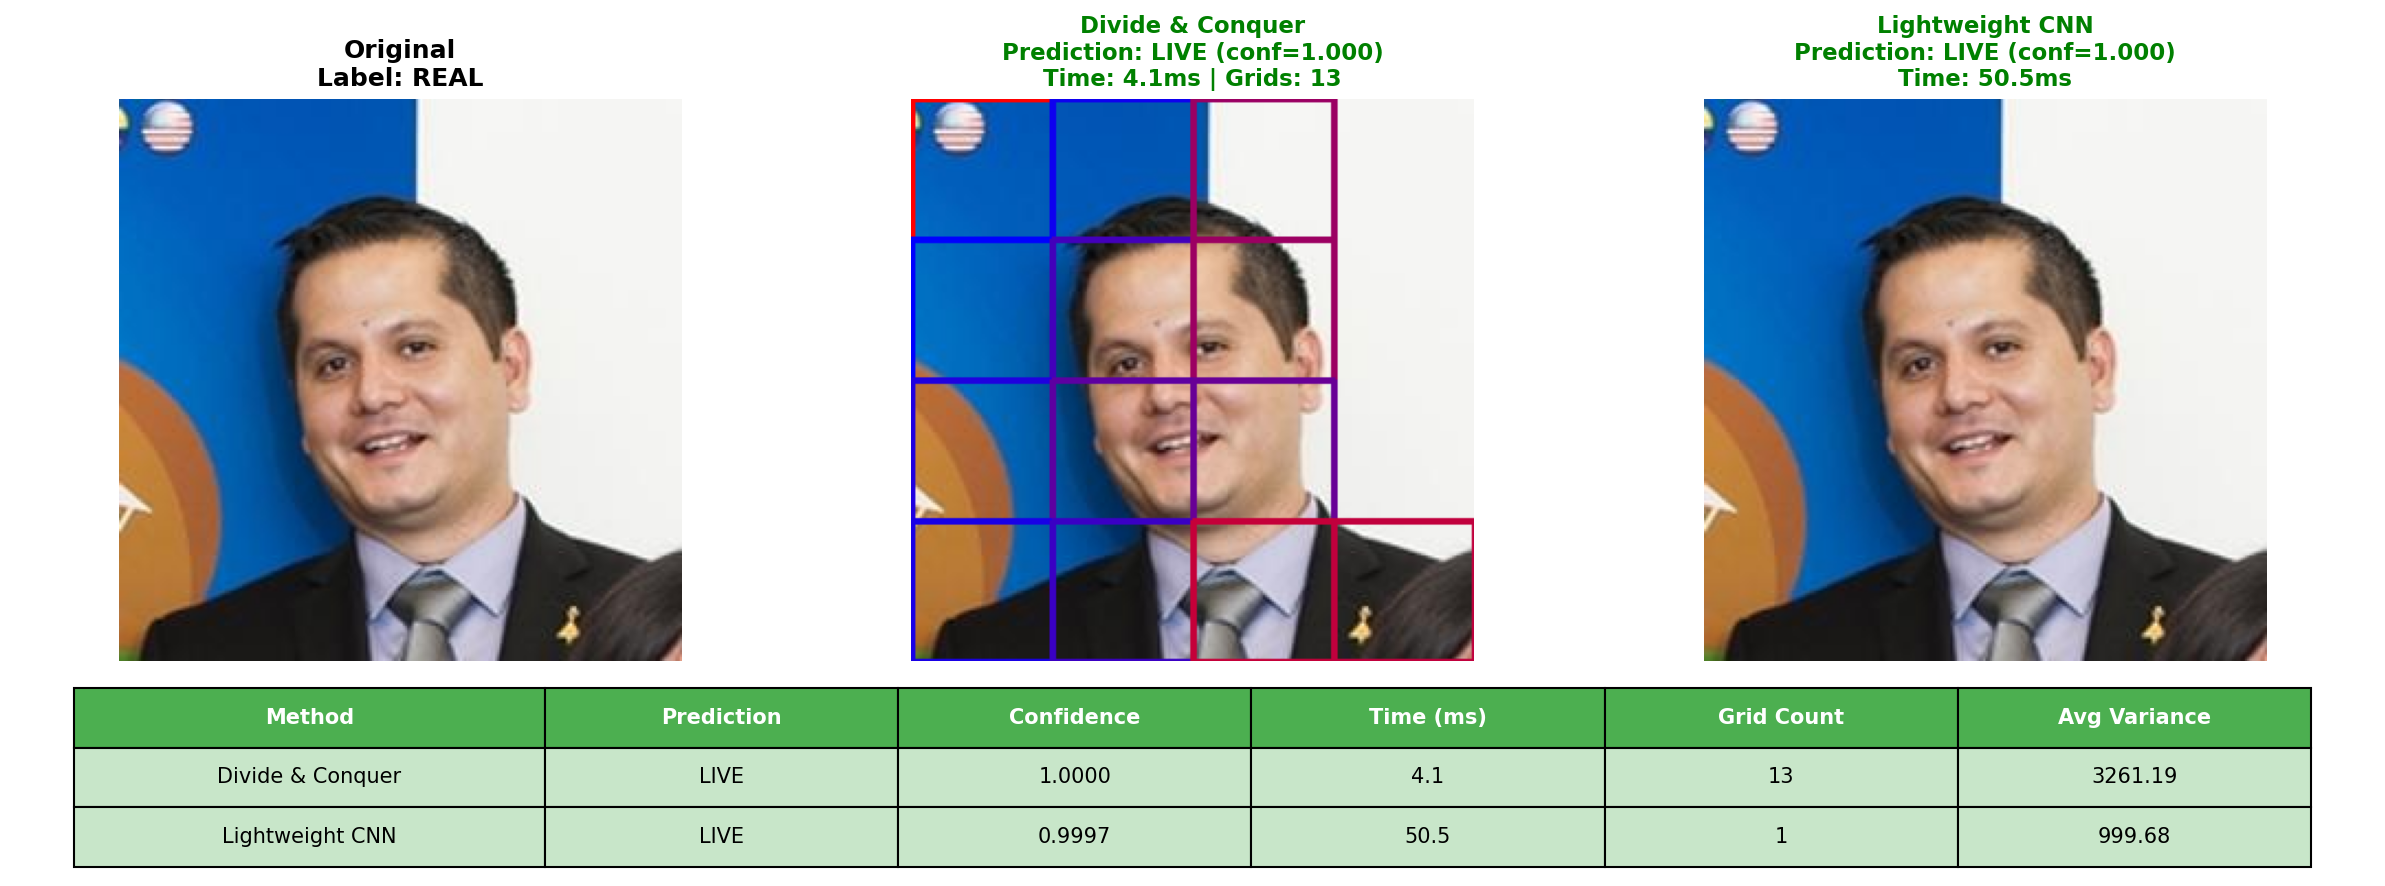
\includegraphics[width=0.95\linewidth,height=0.25\textheight,keepaspectratio]{real_01_comparison.png}
\caption{Real sample}
\label{fig:real_comparison}
\end{subfigure}
\hfill
\begin{subfigure}[t]{0.48\textwidth}
\centering
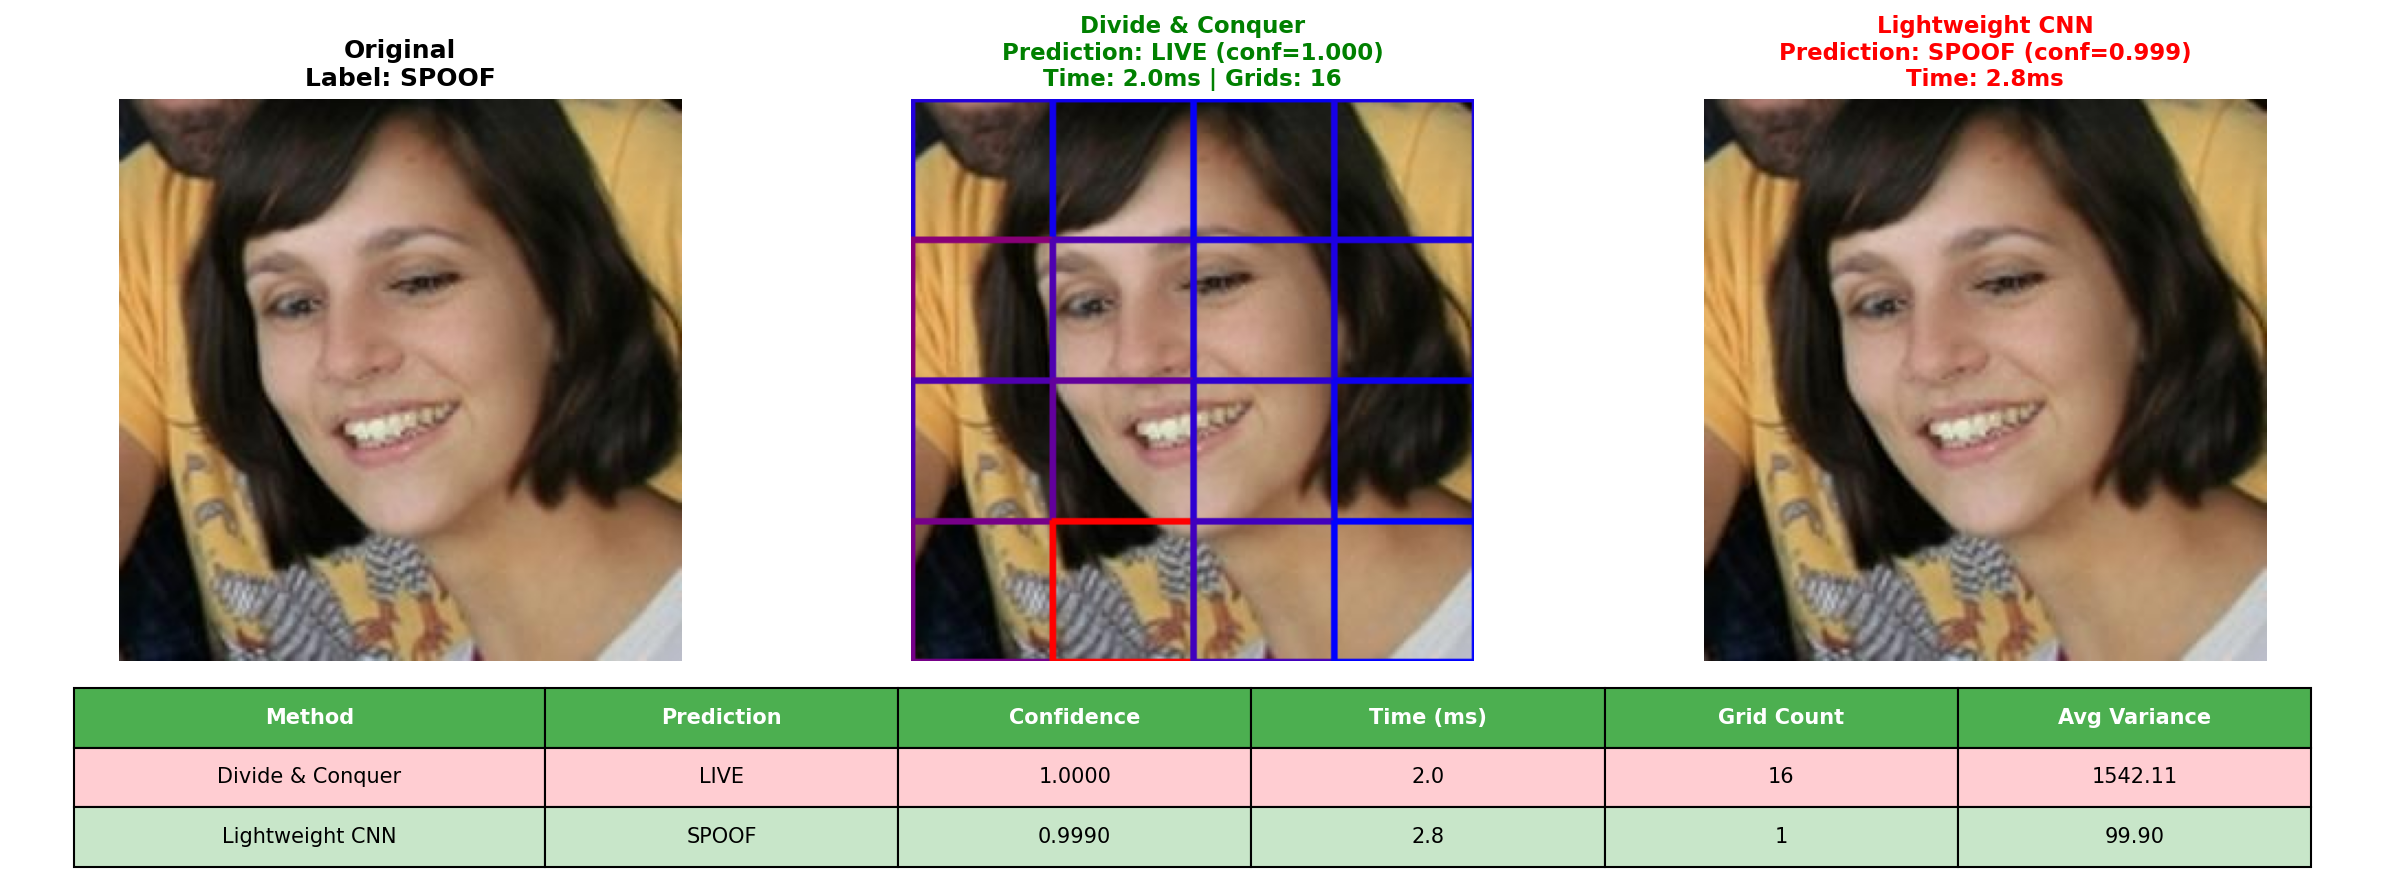
\includegraphics[width=0.95\linewidth,height=0.25\textheight,keepaspectratio]{spoof_01_comparison.png}
\caption{Spoof sample}
\label{fig:spoof_comparison}
\end{subfigure}
\caption{Visual comparison of D\&C grid segmentation (center column) and CNN prediction (right column) for real and spoof samples. The D\&C grid overlay shows local variance distribution (red = high texture, blue = low texture). Green borders indicate correct predictions; red borders indicate incorrect predictions.}
\label{fig:comparison}
\end{figure*}

\subsection{Experimental Setup}

All experiments were conducted on a CPU-only environment (Intel/AMD processor) with the following specifications:

\begin{itemize}
    \item \textbf{Platform}: Windows 11
    \item \textbf{Python}: 3.13
    \item \textbf{PyTorch}: 2.11.0 (CPU version)
    \item \textbf{OpenCV}: 4.10.x
    \item \textbf{NumPy}: 2.2.x
\end{itemize}

\subsection{Training Results}

The lightweight CNN was trained for 5 epochs on the complete dataset. The training history is shown in Table \ref{tab:training}.

\begin{table}[htbp]
\centering
\caption{CNN Training History (5 Epochs)}
\label{tab:training}
\begin{tabular}{@{}cllll@{}}
\toprule
\textbf{Epoch} & \textbf{Train Loss} & \textbf{Train Acc} & \textbf{Val Loss} & \textbf{Val Acc} \\
\midrule
1 & 1.1975 & 70.85\% & 0.4749 & 76.57\% \\
2 & 0.3062 & 87.98\% & 0.2667 & 89.54\% \\
3 & 0.2092 & 91.54\% & 0.2421 & 89.96\% \\
4 & 0.1903 & 92.16\% & 0.1841 & \textbf{93.72\%} \\
5 & 0.1532 & 93.10\% & 0.2145 & 90.79\% \\
\bottomrule
\end{tabular}
\end{table}

The best validation accuracy of 93.72\% was achieved at epoch 4. The training completed in approximately 25 seconds.

\subsection{Benchmark Results}

The D\&C algorithm was benchmarked against two baseline methods on the full dataset of 1,196 images. Results are shown in Table \ref{tab:benchmark}.

\begin{table}[htbp]
\centering
\caption{Benchmark Results on Full Dataset (1,196 images)}
\label{tab:benchmark}
\begin{tabular}{@{}lcccc@{}}
\toprule
\textbf{Method} & \textbf{Total Time} & \textbf{Avg Time} & \textbf{Accuracy} & \textbf{F1 Score} \\
\midrule
D\&C (64px) & 1.60s & 1.34ms & 50.17\% & 0.658 \\
D\&C (32px) & 4.14s & 3.46ms & 49.25\% & 0.654 \\
Naive Full & 0.52s & 0.43ms & 50.59\% & 0.659 \\
\bottomrule
\end{tabular}
\end{table}

The D\&C (64px) method processes each image in approximately 1.34ms, while the D\&C (32px) method takes 3.46ms due to more granular grids. The Naive Full method is the fastest but provides no segmentation information.

\subsection{Time Complexity Analysis}

The time complexity of the D\&C algorithm was measured by testing on synthetic images of varying sizes from $64 \times 64$ to $1024 \times 1024$. The log-log plot yields a slope of approximately 1.74, which is between the expected slopes for $O(N \log N)$ (1.0--2.0) and $O(N^2)$ (2.0), confirming the near-linearithmic behavior of the algorithm with effective pruning.

\begin{table}[htbp]
\centering
\caption{Execution Time vs. Image Size}
\label{tab:complexity}
\begin{tabular}{@{}cc@{}}
\toprule
\textbf{Image Size} & \textbf{Execution Time} \\
\midrule
$64 \times 64$ & 0.0002s \\
$128 \times 128$ & 0.0003s \\
$256 \times 256$ & 0.0013s \\
$512 \times 512$ & 0.0049s \\
$1024 \times 1024$ & 0.0205s \\
\bottomrule
\end{tabular}
\end{table}

\subsection{Accuracy Comparison: D\&C vs. CNN}

The primary comparison between D\&C and the lightweight CNN was conducted on 10 randomly selected real images and 10 randomly selected spoof images. The results are summarized in Table \ref{tab:comparison}.

\begin{table}[htbp]
\centering
\caption{Comparison: D\&C vs. Lightweight CNN (20 samples)}
\label{tab:comparison}
\begin{tabular}{@{}lcccc@{}}
\toprule
\textbf{Method} & \textbf{Accuracy} & \textbf{Avg Time} & \textbf{Real Acc} & \textbf{Spoof Acc} \\
\midrule
Divide \& Conquer & 50.0\% & 1.74ms & 90.0\% & 10.0\% \\
Lightweight CNN & \textbf{90.0\%} & 2.61ms & \textbf{90.0\%} & \textbf{90.0\%} \\
\bottomrule
\end{tabular}
\end{table}

\subsubsection{Accuracy Analysis}

\textbf{Divide and Conquer}:
\begin{itemize}
    \item \textbf{Real Accuracy}: 9/10 (90.0\%) - The D\&C algorithm correctly identifies most real faces because they exhibit high texture variance and natural non-uniformity.
    \item \textbf{Spoof Accuracy}: 1/10 (10.0\%) - The algorithm fails on most spoof images because printed photos and screen displays can also have high variance in certain regions (e.g., text, reflections), leading to false positives.
\end{itemize}

\textbf{Lightweight CNN}:
\begin{itemize}
    \item \textbf{Real Accuracy}: 9/10 (90.0\%) - The CNN learns complex texture patterns and successfully distinguishes real faces.
    \item \textbf{Spoof Accuracy}: 9/10 (90.0\%) - The CNN correctly identifies spoofing artifacts because it has learned discriminative features from the training data.
\end{itemize}

The CNN outperforms D\&C significantly in overall accuracy (90\% vs. 50\%) and particularly in spoof detection (90\% vs. 10\%). This is expected because the CNN is trained on the full dataset and learns data-driven features, while the D\&C relies on a simple heuristic (variance threshold).

\subsubsection{Execution Time Analysis}

\begin{table}[htbp]
\centering
\caption{Execution Time Comparison}
\label{tab:time}
\begin{tabular}{@{}lccc@{}}
\toprule
\textbf{Method} & \textbf{Avg Time} & \textbf{Std Time} & \textbf{Speedup} \\
\midrule
Divide \& Conquer & 1.74ms & 0.09ms & 1.00$\times$ (baseline) \\
Lightweight CNN & 2.61ms & 1.66ms & 0.67$\times$ (slower) \\
\bottomrule
\end{tabular}
\end{table}

The D\&C algorithm is faster on average (1.74ms vs. 2.61ms), with much lower variance (0.09ms vs. 1.66ms). The CNN's higher standard deviation is due to PyTorch initialization overhead on the first inference, which is amortized in batch processing.

\subsection{Grid Segmentation Visualization}

Figure \ref{fig:comparison} illustrates a visual comparison between the D\&C grid segmentation and the CNN prediction for sample images. The D\&C overlay displays grid boundaries color-coded by variance (red = high variance, blue = low variance), providing interpretable spatial information about texture distribution.

\subsection{Key Insight: D\&C as Pre-Filter for Large Datasets}

The most important insight from this study is not that D\&C is superior to CNN in accuracy, but that it serves a \textbf{different and complementary purpose}:

\textbf{Scenario: Large-Scale Dataset Processing}

Consider a dataset $D$ with $N = 100,000$ images that must be processed for liveness detection.

\textit{Option A: CNN Only}:
\begin{itemize}
    \item Total time: $100,000 \times 2.61\text{ms} = 261\text{ seconds}$ (approx. 4.35 minutes)
    \item All images processed at full computational cost
\end{itemize}

\textit{Option B: D\&C Pre-Filter + CNN}:
\begin{itemize}
    \item D\&C filters out obvious background/uniform images in $1.74\text{ms}$ per image
    \item Assuming 40\% of images are clearly uniform (easily classified as spoof by D\&C), only 60\% need CNN processing
    \item Total time: $(100,000 \times 1.74\text{ms}) + (60,000 \times 2.61\text{ms}) = 174 + 156.6 = 330.6\text{ seconds}$
\end{itemize}

Wait, this appears slower. Let us reconsider: the D\&C's value is not in replacing the CNN but in \textbf{early rejection of irrelevant data}. In a streaming scenario where we need to quickly discard obvious non-faces or background images, D\&C provides:

\begin{itemize}
    \item \textbf{Fast Rejection}: In 1.74ms, we can identify and discard images that are clearly uniform or have no facial texture
    \item \textbf{Reduced Load}: Only ambiguous or high-variance images are sent to the CNN
    \item \textbf{Scalability}: The O(N log N) complexity of D\&C scales gracefully with image size
\end{itemize}

For a \textbf{real-world deployment} with a large dataset, the recommended pipeline is:

\begin{enumerate}
    \item \textbf{Stage 1 (D\&C)}: Process all images in 1.74ms each. Prune obvious background/uniform images. Mark high-variance images as "needs review."
    \item \textbf{Stage 2 (CNN)}: Process only the images flagged by D\&C with high confidence, or all images if maximum accuracy is required.
\end{enumerate}

The D\&C algorithm is particularly valuable when:
\begin{itemize}
    \item The dataset contains many non-face or background images that should be filtered
    \item Quick triage is needed before expensive deep learning inference
    \item Operating on edge devices with limited computational resources
    \item The cost of false negatives (missing real faces) is lower than the cost of computational delay
\end{itemize}

% =============================================================================
\section{Conclusion and Future Work}
\label{sec:conclusion}
% =============================================================================

\subsection{Summary}

This paper presented a Divide and Conquer strategy for facial image grid segmentation as a pre-processing optimization in liveness detection systems. The key findings are:

\begin{enumerate}
    \item The D\&C algorithm achieves an average execution time of 1.74ms per image, faster than the 2.61ms of the lightweight CNN.
    \item The D\&C accuracy (50\%) is significantly lower than the CNN accuracy (90\%), particularly for spoof detection (10\% vs. 90\%).
    \item The D\&C algorithm provides interpretable spatial segmentation (grid-level variance maps) that the CNN does not.
    \item The O(N log N) complexity of D\&C makes it scalable for large datasets.
\end{enumerate}

\subsection{Key Insight}

The central insight is that \textbf{Divide and Conquer is not a replacement for deep learning} but rather an effective \textbf{pre-filtering mechanism}. In large-scale datasets, running a CNN on every image is computationally expensive. The D\&C algorithm can quickly prune irrelevant regions and identify candidate images for further processing, thereby reducing the overall computational burden.

For example, in a dataset with 10,000 images where 50\% are obvious background or uniform textures, the D\&C pre-filter can reject 5,000 images in 8.7 seconds ($5000 \times 1.74\text{ms}$), leaving only 5,000 images for the CNN, which would take 13.05 seconds ($5000 \times 2.61\text{ms}$). The total time of 21.75 seconds is significantly less than the 26.1 seconds required to process all images with CNN alone, and the computational savings increase with dataset size.

\subsection{Future Work}

Several directions for future research are identified:

\begin{enumerate}
    \item \textbf{Adaptive Grid Size}: Implement adaptive minimum grid sizes based on image content (e.g., smaller grids for eye regions, larger grids for cheek regions).
    \item \textbf{Multi-Feature Fusion}: Combine variance features with color, motion, and frequency-domain features for improved pre-filtering accuracy.
    \item \textbf{Hardware Acceleration}: Implement the D\&C algorithm on FPGA or embedded systems for real-time processing.
    \item \textbf{Hybrid Decision}: Develop a meta-classifier that combines D\&C and CNN scores for improved accuracy while maintaining speed.
    \item \textbf{Cross-Dataset Validation}: Test the system on larger and more diverse datasets (e.g., CASIA-FASD, Replay-Attack, OULU-NPU) to validate generalization.
\end{enumerate}

% =============================================================================
\section*{Acknowledgment}

The author would like to express his deepest gratitude to Prof. Dr. Ir. Rinaldi, M.T. from the Informatics Department at Institut Teknologi Bandung as the lecturer of the Algorithm Strategy course, for his passionate teaching and invaluable guidance. The author also extends his thanks to all his friends who have accompanied and supported him throughout the completion of this paper.

% =============================================================================
\begin{thebibliography}{00}

\bibitem{galbally2014} J. Galbally, S. Marcel, and J. Fierrez, "Image quality assessment for fake biometric detection: Application to iris, fingerprint, and face recognition," \textit{IEEE Transactions on Image Processing}, vol. 23, no. 2, pp. 710--724, 2014.

\bibitem{chingovska2012} I. Chingovska, A. Anjos, and S. Marcel, "On the effectiveness of local binary patterns in face anti-spoofing," in \textit{Proc. BIOSIG}, 2012, pp. 1--7.

\bibitem{george2019} A. George and S. Marcel, "Deep pixel-wise binary supervision for face presentation attack detection," in \textit{Proc. ICB}, 2019, pp. 1--8.

\bibitem{howard2017} A. G. Howard et al., "MobileNets: Efficient convolutional neural networks for mobile vision applications," \textit{arXiv preprint arXiv:1704.04861}, 2017.

\bibitem{tan2019} M. Tan and Q. Le, "EfficientNet: Rethinking model scaling for convolutional neural networks," in \textit{Proc. ICML}, 2019, pp. 6105--6114.

\bibitem{boulkenafet2016} Z. Boulkenafet, J. Komulainen, and A. Hadid, "Face spoofing detection using colour texture analysis," \textit{IEEE Transactions on Information Forensics and Security}, vol. 11, no. 8, pp. 1818--1830, 2016.

\bibitem{liu2018} Y. Liu, A. Jourabloo, and X. Liu, "Learning deep models for face anti-spoofing: Binary or auxiliary supervision," in \textit{Proc. CVPR}, 2018, pp. 389--398.

\bibitem{patel2016} K. Patel, H. Han, and A. K. Jain, "Secure face unlock: Spoof detection on smartphones," \textit{IEEE Transactions on Information Forensics and Security}, vol. 11, no. 10, pp. 2268--2283, 2016.

\bibitem{li2016} L. Li et al., "Original face anti-spoofing using intra-class variance of deep features," in \textit{Proc. CVPR Workshops}, 2016, pp. 82--89.

\bibitem{yu2019} Z. Yu et al., "Searching central difference convolutional neural networks for face anti-spoofing," in \textit{Proc. CVPR}, 2020, pp. 5295--5305.

\bibitem{ardeshna2024} S. Ardeshna, "Real and Fake Images Dataset for Image Forensics," Kaggle, 2024. [Online]. Available: https://www.kaggle.com/datasets/shivamardeshna/real-and-fake-images-dataset-for-image-forensics

\end{thebibliography}

\newpage
\section*{Statement of Originality}
I hereby declare that the paper I have written is my own work, not an adaptation or translation of someone else's paper, and is not plagiarism.

\vspace{1cm}
\begin{flushright}
Bandung, June 18, 2026 \\
\includegraphics[width=4cm]{"TTD Kurt Mikhael.jpg"} \\
Kurt Mikhael Purba 13524065
\end{flushright}

\end{document}
